%% ---------------------------------------------------------------------------
%% Manuscript: field-realisable SOH over a BMS, with measured evidence sufficiency
%% Class: Elsevier elsarticle (Journal of Energy Storage / Reliability
%% Engineering & System Safety). Compile with pdflatex + bibtex (e.g. Overleaf).
%%
%% STATUS: DRAFT. Every \citeneeded{} renders in red and is an open citation
%% gap that must be filled from a documented survey - never from memory.
%% Every number traces to an artifact under reports/metrics/ (Appendix A).
%% ---------------------------------------------------------------------------
\documentclass[preprint,12pt,authoryear]{elsarticle}

\usepackage{amsmath,amssymb}
\usepackage{booktabs}
\usepackage{graphicx}
\usepackage{xcolor}
\usepackage[hidelinks]{hyperref}
\usepackage{lineno}

\newcommand{\citeneeded}[1]{\textcolor{red}{[CITE: #1]}}
\newcommand{\SOH}{\mathrm{SOH}}
\newcommand{\Qw}{Q_{\mathrm{w}}}

\journal{Journal of Energy Storage}

\begin{document}

\begin{frontmatter}

\title{Measuring lithium-ion cell health from voltage, current and time:
a validated software layer over the battery management system, and when its
evidence suffices}

\author[inst1]{Naveen Vaidyanathan\corref{cor1}}
\ead{[EMAIL]}
\cortext[cor1]{Corresponding author.}
\affiliation[inst1]{organization={[DEPARTMENT, INSTITUTION]},
            city={[CITY]},
            country={[COUNTRY]}}

\begin{abstract}
A battery management system (BMS) measures terminal voltage, current and
temperature; whether a software layer above it can convert these into a
trustworthy state of health (SOH) is usually answered by fitting a model. On 31
NASA cells in nine protocol cohorts, twelve published methods all lost skill
under leave-one-cohort-out validation, with overlapping intervals,
motivating estimators that fit nothing across cells. We estimate SOH as the
ratio of charge delivered within a fixed voltage window to the same quantity on
the cell's own first discharges, correcting ohmic sag with a resistance
identified from the voltage step at each load onset. From voltage, current and
time alone, on 22 CALCE lithium cobalt oxide cells, the median per-cell error
was 1.7\% (95\% CI 1.4--4.3\%) on 17 cells, with five refused for stated
physical causes. The same step resistance tracked the cycler's measured
resistance on 19 of 20 cells (median Spearman 0.86). For partial cycling, a
window learned from each cell's early discharges achieved 3.2--3.4\% error,
while windows on the discharge knee were refused by a steepness criterion.
Remaining useful life extrapolated from each cell's own fade was within
$\pm$20 cycles 73\% of the time in the last 25 cycles before 90\% capacity;
predictions under 25 cycles were not exceeded in 95\% of cases. Evidence
sufficiency was measured rather than assumed: the number of observed
discharges did not predict accuracy, whereas the trend-removed consistency of
readings did (1.3\% versus 5.1\% median error). Each output is
validated, banded by its measured error, or refused.
\end{abstract}

\begin{highlights}
\item SOH from voltage, current and time alone: 1.7\% median error on 17 CALCE cells
\item Load-step resistance tracks laboratory resistance on 19 of 20 cells
\item Partial-discharge SOH at 3.2--3.4\%; windows on the discharge knee are refused
\item Consistency of readings, not their count, predicts estimate accuracy
\item Twelve fitted models lose skill when the test protocol changes
\end{highlights}

\begin{keyword}
lithium-ion battery \sep state of health \sep battery management system \sep
internal resistance \sep partial discharge \sep remaining useful life \sep
uncertainty quantification
\end{keyword}

\end{frontmatter}

\linenumbers

%% ===========================================================================
\section{Introduction}
\label{sec:intro}

A battery management system (BMS) protects a pack and estimates its state of
charge. It already holds the three measurements from which ageing is visible:
terminal voltage, current and temperature. A software layer above it can, in
principle, turn them into answers an operator acts on: how much of its original
capacity the battery retains, how fast that is changing, and when it should be
replaced.

The dominant way to build that layer is to fit a model. Features are
extracted from cycling data and a regressor is trained to predict SOH
\citeneeded{reviews of data-driven SOH estimation}, with feature sets ranging
from usage aggregates to discharge-curve descriptors such as the
capacity--voltage difference between cycles \citep{severson2019}. Skill is
commonly reported under leave-one-cell-out validation, in which a held-out
cell's siblings from the same test protocol remain in training, so the test
asks whether the model recognises a protocol it has already seen. Group-wise
splitting by cell changes reported skill substantially \citep{maher2025}, and
a large gap between random and cell-wise splits has been reported on NASA data
\citep{le2026}.

A deployed BMS faces a harder question: the next battery comes from
conditions the training set never contained. Section~\ref{sec:res-bench}
shows that, on the data available to us, no fitted method retains reliable
skill under that question, and no method can be distinguished from another.
We take that as the starting point and ask what a software layer \emph{can}
measure reliably from the BMS's own signals, how accurately, and when it should
decline to answer.

\subsection{Contributions}
\begin{enumerate}
\item A field-realisable SOH estimator validated from voltage, current and time
alone, in which the ohmic correction uses a resistance identified from the
voltage step at each load onset. Relative to no correction, this raises
coverage from 12 to 17 of 22 cells and lowers median error from 4.3\% to
1.7\% (Section~\ref{sec:res-field}).
\item Resistance as a validated second health quantity: the step resistance
tracks the laboratory instrument on 19 of 20 cells (Section~\ref{sec:res-r}).
\item SOH from partial discharges via a window learned from the cell's own early
discharges, with a physical refusal rule for windows on the discharge knee whose
threshold is not tuned (Section~\ref{sec:res-partial}).
\item Remaining-useful-life (RUL) accuracy reported as a user meets it, indexed
by the prediction, together with a measured correction (88\% $\to$ 73\%) caused
by a reference capacity that used the future (Section~\ref{sec:res-rul}).
\item Evidence sufficiency measured rather than asserted: confidence follows the
consistency of readings, which predicts error, not the number of discharges,
which does not (Section~\ref{sec:res-suff}).
\item Negative results retained: fitted models across protocols
(Section~\ref{sec:res-bench}) and four routes to RUL from sparse complete
discharges (Section~\ref{sec:res-sparse}).
\end{enumerate}

\subsection{Scope}
All validation is on single cells of one lithium cobalt oxide (LCO) family at
constant current. The paper makes no claim about packs, other chemistries or
dynamic drive cycles, does not correct temperature-dependent capacity (the
CALCE cycling records carry no temperature channel), and validates end of life
at 90\% rather than the 80\% automotive convention, because the CALCE
trajectories end near 81\%. A bench rig validates data acquisition, not health
estimation.

%% ===========================================================================
\section{Related work}
\label{sec:related}

\noindent\textcolor{red}{[To be written from a documented survey. Every claim
below needs a verified reference.]}

\paragraph{Data-driven SOH and validation practice}
Feature-based regressors and sequence models dominate
\citeneeded{reviews}. The split used for validation changes reported skill
\citep{maher2025,le2026}.

\paragraph{Discharge-curve and partial-segment estimators}
Capacity--voltage difference features \citep{severson2019}, incremental
capacity and differential voltage analysis \citeneeded{ICA/DVA methods}, and
estimators built on partial charge or discharge segments
\citeneeded{partial-segment SOH methods}. The present estimator belongs to the
last family. The distinctions to establish against it are: no cross-cell
fitting; an online resistance correction from the load step; gates that refuse
rather than extrapolate; and validation from raw telemetry rather than cycler
summaries.

\paragraph{Online resistance identification}
Pulse- and step-based resistance estimation in BMS
\citeneeded{online resistance identification}. Here it serves both as a
correction and as a reported output.

\paragraph{Prognostics and uncertainty}
RUL estimation and its uncertainty \citeneeded{RUL reviews; prognostic
uncertainty}.

%% ===========================================================================
\section{Data}
\label{sec:data}

\paragraph{CALCE CS2 and CX2}
Prismatic LCO cells cycled at room temperature \citep{calce}: CS2 rated
1.1~Ah (Type~1: 0.9~Ah) and CX2 rated 1.35~Ah, grouped by the dataset's test
types. We use the 22 cells for which raw cycler records and full-discharge
capacity are available. They include:
\begin{itemize}
\item constant-current cycling at several rates;
\item multi-rate cycling (Type~3), whose discharge switches rate within a cycle;
\item real partial cycling (CS2 Types 5 and 6): thousands of ${\sim}$25\%-depth
discharges in a fixed band, with a full capacity check roughly every 100
cycles. Type~6 cycles at the top of charge (${\sim}$4.07$\to$3.78~V); Type~5
near empty (${\sim}$3.69$\to$2.70~V).
\end{itemize}
Records span many files whose test time restarts per file. A monotonic time base
is constructed by offsetting each restart rather than by sorting timestamps,
which would interleave overlapping segments.

\paragraph{NASA PCoE}
18650 cells under nine documented protocols (ambient ${\sim}$4--43~$^\circ$C,
varied loads and cut-offs) \citep{saha2007}, used only for the benchmark of
Section~\ref{sec:res-bench}: 31 cells after admissibility screening, 2{,}585
cycle-level rows, nine cohorts.

\paragraph{Bench rig}
An ESP8266 microcontroller with an INA219 current/voltage monitor and an LM35
temperature sensor on a single 18650 cell, streaming a checksummed line
protocol at 1~Hz (Section~\ref{sec:res-system}).

%% ===========================================================================
\section{Methods}
\label{sec:methods}

\subsection{From telemetry to discharges}
The estimator receives voltage $V(t)$, current $I(t)$ and time; the cycler's
capacity, resistance and cycle summaries are removed before scoring. Current is
segmented into charge, discharge and rest phases using a dead band (0.02~A for
CALCE, where rest is logged as exactly zero) and a minimum run length. The
charge delivered on discharge $n$ is the trapezoidal integral of $|I|\,dt$.
Every discharge is retained: a partial discharge that crosses the window is a
full measurement of the window.

\subsection{Voltage-window state of health}
For a window $[V_\mathrm{low}, V_\mathrm{high}]$, the window charge
$\Qw(n)$ is the charge delivered while terminal voltage falls from
$V_\mathrm{high}$ to $V_\mathrm{low}$ on discharge $n$. It is read by
interpolation, and requires that the discharge span at least 95\% of the
window. With $\mathcal{R}$ the cell's first five measurable discharges,
\begin{equation}
\SOH(n) = \frac{\Qw(n)}{\operatorname{median}_{m\in\mathcal{R}} \Qw(m)} ,
\label{eq:soh}
\end{equation}
and the reported value is the median of the latest five accepted readings. The
primary window, 3.90--3.60~V, was fixed before any validation run;
4.05--3.55 and 3.85--3.55~V are reported as sensitivity analyses, not
selected between.

Eq.~\eqref{eq:soh} assumes the discharge curve scales approximately uniformly
with capacity. Loss of lithium inventory shifts the curve, which the ratio
partly absorbs. Loss of active material and resistance growth change its shape
and position, which it does not. This is the method's principal approximation;
Section~\ref{sec:res-suff} measures how it drifts with age.

\subsection{Resistance from the load step and ohmic correction}
Under load, terminal voltage lies below open-circuit voltage by approximately
$IR$. As $R$ grows with age, a fixed terminal-voltage window slides along the
curve, and the slide reads as additional fade. At each discharge onset,
between the last rest sample and the first loaded sample,
\begin{equation}
R_\mathrm{step} = \frac{V_\mathrm{rest} - V_\mathrm{load}}{|I_\mathrm{load} - I_\mathrm{rest}|},
\label{eq:rstep}
\end{equation}
accepted when the two samples are within 60~s and the current change is at
least 0.05~A. $R_\mathrm{step}$ is an \emph{apparent} resistance: the ohmic
drop plus polarisation accrued by the first loaded sample. On cell CS2\_35 it
is ${\sim}0.165~\Omega$ against the cycler's ${\sim}0.099~\Omega$. Each
discharge uses the trailing median $\tilde R(n)$ of the last 11 step estimates,
so no correction depends on later data, and its window is shifted to
\begin{equation}
[V_\mathrm{low} - |I_n|\tilde R(n),\; V_\mathrm{high} - |I_n|\tilde R(n)] .
\label{eq:shift}
\end{equation}
Discharges preceding the first resistance estimate are left unmeasured rather
than scored uncompensated.

\subsection{Gates}
Each gate needs no ground truth and can therefore run in deployment.
\begin{enumerate}
\item \emph{Truncated discharge.} A discharge delivering less than 50\% of the
reference discharges' total charge is not scored; a cut-short cycle crosses the
window with little charge and would read as severe fade.
\item \emph{Physical plausibility.} A ratio below 0.50 is withheld, and a cell
with more than 20\% of readings below it is refused entirely. A ratio above
1.10 is withheld as not spanning the same part of the curve.
\item \emph{Reference timing.} The reference must be complete within 20
equivalent full cycles of charge throughput. Throughput rather than a
discharge count is used because storage-protocol records contain thousands of
short pulses.
\end{enumerate}

\subsection{Learned windows for partial discharges}
When the fixed window cannot be read and the rated capacity $C_\mathrm{rated}$
is known, a window is learned from the cell's first ten discharges only. The
band they all cover is trimmed by 15\% at each end, and the flattest sub-window
of up to 0.30~V within it is selected by its steepness
\begin{equation}
s = \frac{V_\mathrm{high}-V_\mathrm{low}}{\Qw/C_\mathrm{rated}}
\quad [\mathrm{V\ per\ unit\ state\ of\ charge}] .
\label{eq:steep}
\end{equation}
The window is refused if even the flattest choice has $s > 2.0$, because it
then lies on the end-of-discharge knee. There, voltage reflects kinetics
(resistance and solid-state diffusion) rather than stored charge.

\subsection{RUL from the cell's own fade}
At cycle $k$, the cell's SOH history up to $k$ is smoothed with an 11-point
rolling median, a straight line is fitted to the full history, and its crossing
of 0.90 gives the end-of-life estimate. Estimates are refused in four cases:
with fewer than 30 points; for flat or rising trends; and when the estimate
reaches more than twice the history length ahead. A cell already past the
threshold is reported as zero. Linear, square-root and quadratic forms, over
full and trailing windows, were compared; the full-history line was most
accurate near end of life.

\subsection{Evidence sufficiency}
Each output has its own requirements:
\begin{itemize}
\item capacity health: voltage, current, and five reference readings plus one;
\item resistance health: a clean load step;
\item RUL: 30 complete discharges;
\item heat exposure: a temperature channel.
\end{itemize}
Within capacity health, confidence follows consistency. Because a healthy
estimate keeps changing as the cell ages, stability of the estimate is the
wrong criterion; the question is whether readings agree once that trend is
removed. With $\sigma_{\tilde x}(x_{1..n}) = 1.2533\,\mathrm{MAD}(x)/\sqrt{n}$
the standard error of a median,
\begin{align}
u_\mathrm{ref} &= \frac{\sigma_{\tilde x}\!\left(\Qw(\mathcal{R})\right)}{\operatorname{median}\Qw(\mathcal{R})}, \\
u_\mathrm{rec} &= \frac{1.2533\,\mathrm{MAD}(\varepsilon)}{\sqrt{5}}, \\
u &= \sqrt{u_\mathrm{ref}^2 + u_\mathrm{rec}^2},
\label{eq:u}
\end{align}
where $\varepsilon$ are the residuals of the last ten readings about their own
straight line. The tolerance $u \le 0.01$ (one SOH point) was fixed before the
study of Section~\ref{sec:res-suff}, chosen to lie below the validated 1.7\%
median error.

\subsection{Validation protocol}
\paragraph{Ground truth}
Ground truth is the cycler's measured discharge capacity, which never enters
an estimate. SOH truth is capacity over the median of the cell's first five
cycles. For partial-cycling cells, whose checks are ${\sim}$100 cycles apart, it
is capacity over the checks within the first ten cycles. This is the reference a
BMS can hold. A reference drawn from the cell's whole record uses the future;
Section~\ref{sec:res-rul} quantifies the resulting inflation.

\paragraph{Pre-declared configurations}
Primary windows, comparison arms, tolerances and scoring were fixed before each
study ran. Choices made after seeing a result are labelled exploratory.

\paragraph{Benchmark}
The benchmark (Section~\ref{sec:res-bench}) uses leave-one-cell-out (LOBO, 31
folds) and leave-one-cohort-out (LOCO, 9 folds) validation. $R^2$ is computed
against the training-fold mean, with 95\% bootstrap intervals resampling folds
(2{,}000 resamples). Hyperparameters were fixed, not tuned per fold, except
ElasticNet's penalty, chosen by inner cross-validation within the training
fold.

\paragraph{Aggregation}
Errors are summarised per cell, then across cells, so long-lived cells do not
dominate.

%% ===========================================================================
\section{Results}
\label{sec:results}

\subsection{Fitted models do not survive a change of protocol}
\label{sec:res-bench}

On the NASA benchmark (target SOH; isotonic signal ceiling 0.569) every one of
twelve methods lost skill from LOBO to LOCO (Table~\ref{tab:bench}). LOBO rank
carried almost no information about LOCO rank (Spearman $\rho = +0.084$,
$p = 0.795$). Across fourteen methods, the spread of LOCO point estimates (2.06
in $R^2$) was smaller than the width of the best method's own interval (3.66).

\begin{table}[t]
\centering
\caption{Benchmark on 31 NASA cells in nine cohorts (six of twelve methods shown).
LOCO intervals are 95\% bootstrap over folds.}
\label{tab:bench}
\begin{tabular}{lrrlr}
\toprule
Method & LOBO $R^2$ & LOCO $R^2$ & LOCO 95\% CI & LOCO MAE \\
\midrule
XGBoost & 0.732 & 0.459 & $[-2.80,\ 0.86]$ & 7.62\% \\
Age-linear baseline & 0.483 & 0.406 & $[-0.43,\ 0.51]$ & 10.71\% \\
ElasticNet & 0.609 & 0.355 & $[-1.65,\ 0.76]$ & 10.31\% \\
GPR (Mat\'ern) & 0.725 & 0.207 & $[-3.72,\ 0.43]$ & 17.06\% \\
Random forest & 0.773 & 0.150 & $[-1.09,\ 0.90]$ & 10.67\% \\
LSTM (10-cycle windows) & 0.594 & $-0.185$ & $[-2.09,\ 0.66]$ & 17.36\% \\
\bottomrule
\end{tabular}
\end{table}

Ablation isolates where the skill comes from:
\begin{itemize}
\item XGBoost on cycle number alone scored LOCO $R^2 = -0.27$;
\item on behaviour features alone, $-0.29$;
\item only their combination reached 0.459, while a straight line on cycle
number reached 0.406.
\end{itemize}
Shuffling each cell's capacity in time placed every LOCO interval at or below
zero, so the harness does not manufacture skill. Usage features thus added
about 0.05 in $R^2$ over counting cycles, within the intervals. Temperature was
the only usage factor with a consistent, correctly signed within-protocol
relationship to fade (seven of seven cells), and its magnitude did not transfer
between protocols.

\subsection{Field SOH from voltage, current and time}
\label{sec:res-field}

Table~\ref{tab:field} compares three ohmic treatments at the primary window on
22 CALCE cells. The field correction matched the laboratory correction within
its interval and measured five more cells. Sensitivity windows gave 1.2\%
(4.05--3.55~V, 16 cells) and 1.9\% (3.85--3.55~V, 17 cells).

\begin{table}[t]
\centering
\caption{Field SOH at the 3.90--3.60~V window; median per-cell absolute error
against cycler capacity, 95\% bootstrap interval over cells.}
\label{tab:field}
\begin{tabular}{lcccc}
\toprule
Ohmic correction & Cells & Median & 95\% CI & Worst \\
\midrule
None & 12/22 & 4.3\% & 2.5--5.4\% & 6.4\% \\
Cycler resistance (laboratory only) & 12/20 & 1.4\% & 1.2--2.5\% & 5.6\% \\
\textbf{Step resistance (field)} & \textbf{17/21} & \textbf{1.7\%} & \textbf{1.4--4.3\%} & \textbf{10.3\%} \\
\bottomrule
\end{tabular}
\end{table}

The three worst cells (6.4--10.3\%) are all Type~3, whose discharge switches
rate within a cycle. Every refusal carries a stated cause:
\begin{itemize}
\item four storage and partial-protocol cells delivered 80--155 equivalent
full cycles before any constant-current discharge crossed the window, so the
reference gate refused them;
\item one cell never rests before discharging, so no step resistance exists.
\end{itemize}
Figure~\ref{fig:track} tracks the estimate against every laboratory capacity
test; Figure~\ref{fig:cells} shows all measured cells.

\begin{figure}[t]
\centering
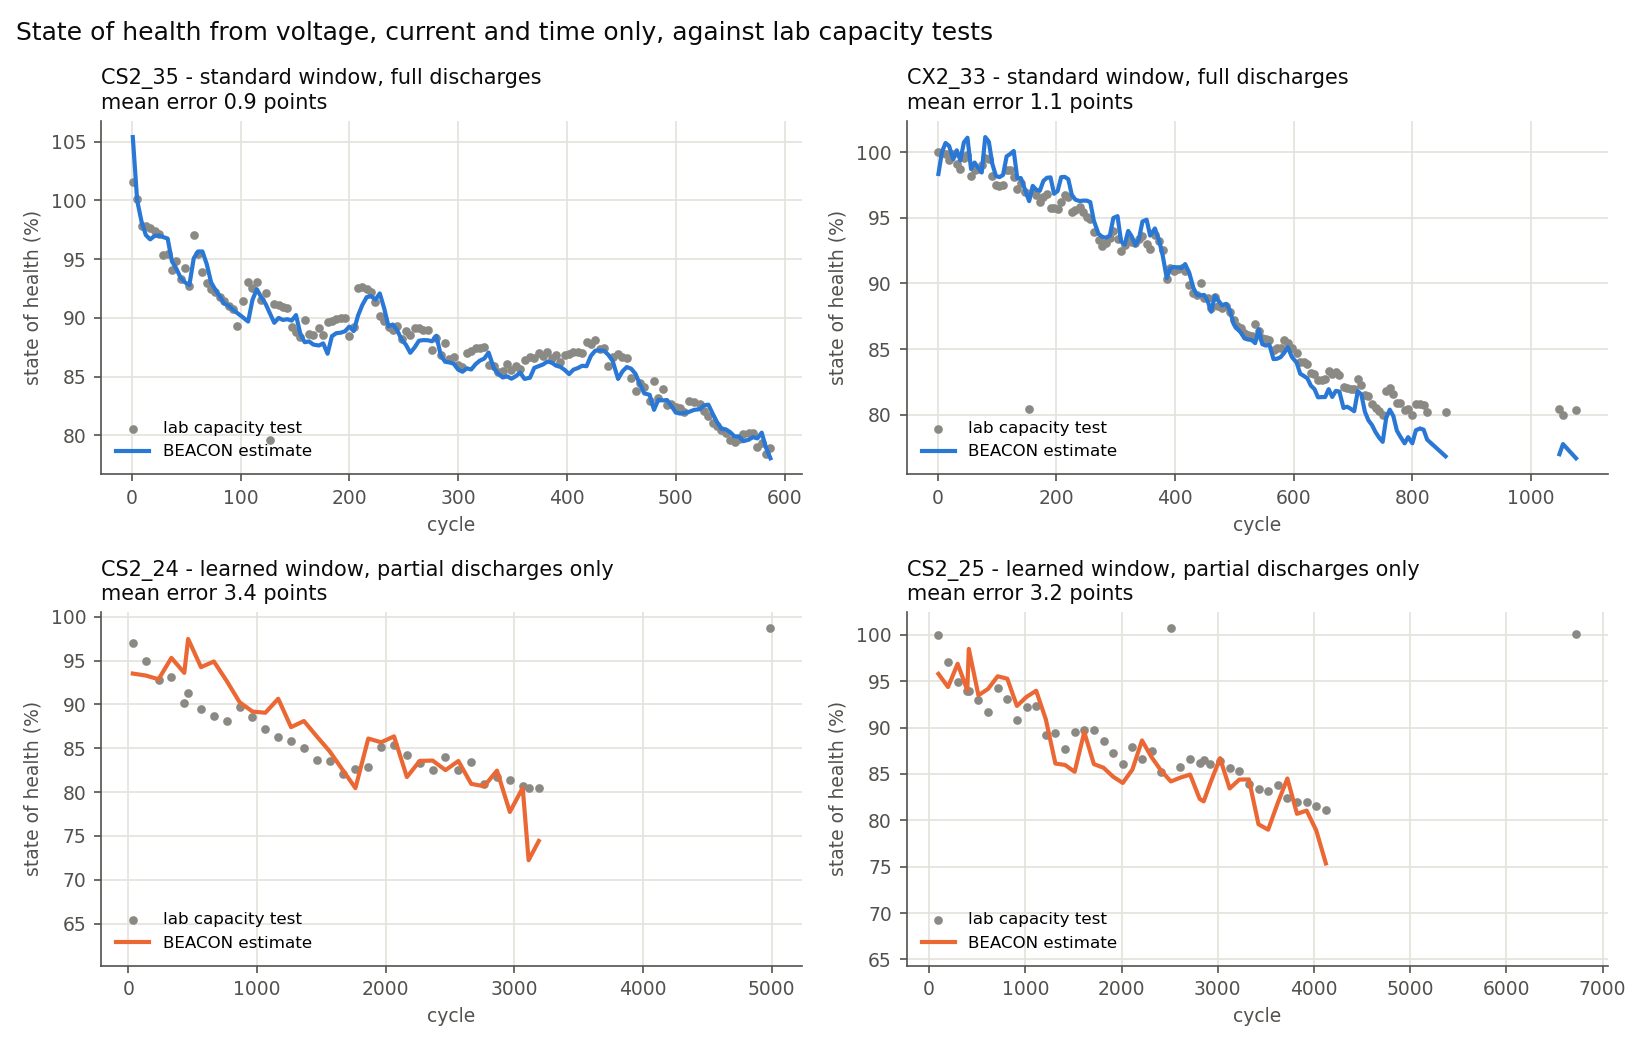
\includegraphics[width=\textwidth]{figures/results_soh_tracking.png}
\caption{SOH from voltage, current and time against every laboratory capacity
test. Top: two constant-current cells, fixed window (mean error 0.9 and 1.1
points). Bottom: two cells of real partial cycling, learned window, estimate
from partial discharges only (3.4 and 3.2 points). Lines are broken across long
gaps without data.}
\label{fig:track}
\end{figure}

\begin{figure}[t]
\centering
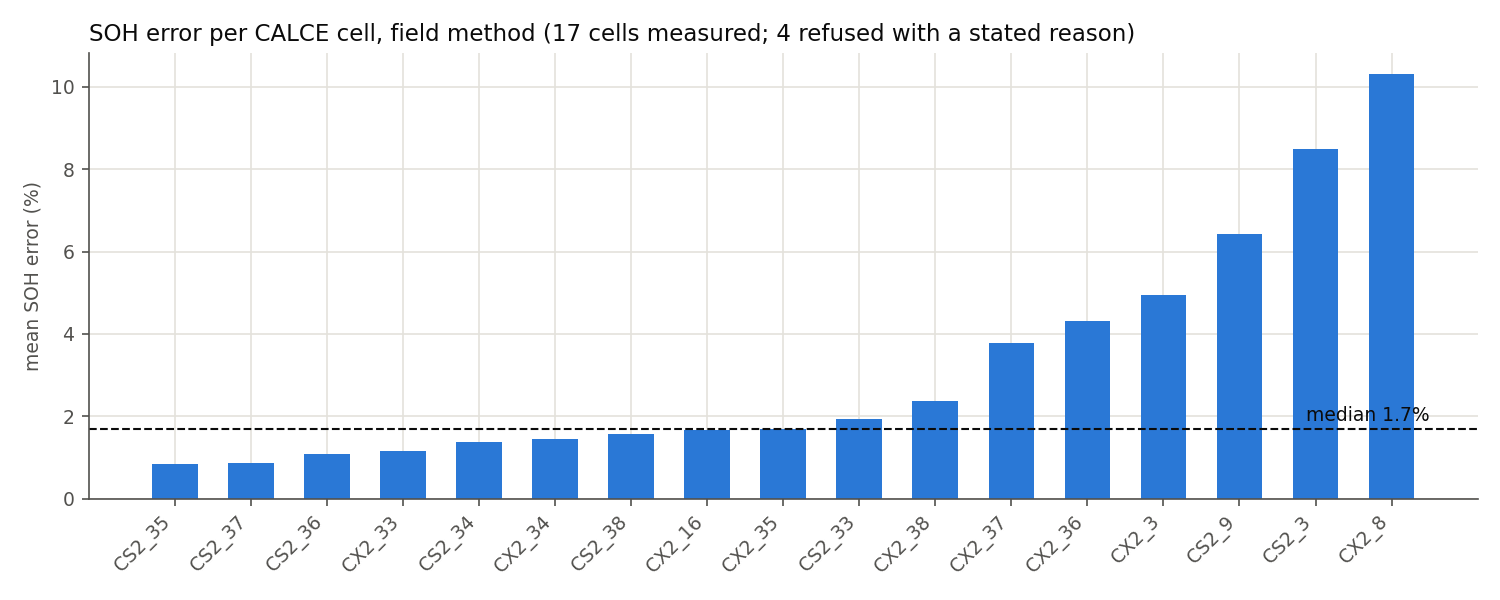
\includegraphics[width=\textwidth]{figures/results_soh_per_cell.png}
\caption{Mean absolute SOH error for every measured CALCE cell, field method;
dashed line is the median (1.7\%).}
\label{fig:cells}
\end{figure}

\subsection{Partial discharges}
\label{sec:res-partial}

On the four cells of real partial cycling (Table~\ref{tab:partial}), estimates
use only partial discharges preceding each laboratory check. Before the knee
gate existed, the two near-empty cells were reported at 6.8\% and 12.8\%. Learned
windows on the 18 full-discharge cells have steepness 0.44--0.88. Any threshold
between about 0.9 and 8 therefore gives the same verdict on every cell, and the
chosen 2.0 is not tuned. As a control, the learned mode on those 18 cells
measured 16 at a median of 1.95\%, beside 1.7\% for the fixed window: it is a
fallback, not a replacement.

\begin{table}[t]
\centering
\caption{SOH from real partial cycling (CALCE CS2 Types 5 and 6).}
\label{tab:partial}
\begin{tabular}{llccl}
\toprule
Cell & Band & Learned window & Steepness & Result \\
\midrule
CS2\_24 & top of charge & 4.00--3.82 V & 0.83 & 3.4\% error \\
CS2\_25 & top of charge & 4.03--3.83 V & 0.82 & 3.2\% error \\
CS2\_5 & near empty & -- & 10.4 & refused (knee) \\
CS2\_6 & near empty & -- & 8.2 & refused (knee) \\
\bottomrule
\end{tabular}
\end{table}

\subsection{Resistance tracks the instrument}
\label{sec:res-r}

Against the cycler's internal-resistance column over each cell's life (20 cells
carrying both values), the step resistance achieved:
\begin{itemize}
\item a median Spearman correlation of 0.86;
\item growth in the same direction on 19 of 20 cells;
\item median growth of 1.26$\times$ versus the cycler's 1.29$\times$.
\end{itemize}
This includes the partial-cycling cells (0.90 and 0.98); the exception is a
Type~3 cell. The levels differ, since the step value includes early
polarisation, but the trends agree, which is what a power-fade indicator
requires.

\subsection{Remaining useful life}
\label{sec:res-rul}

At threshold 0.90, referenced to each cell's first cycles (17 cells),
Table~\ref{tab:rul} reports accuracy by the true distance to end of life and by
the prediction a user sees. Near end of life the estimate is a safe lower
bound: it warns early, almost never late. Errors are predominantly early
because these cells fade quickly at first and then more slowly, so a
full-history line is steeper than the remaining fade.

\begin{table}[t]
\centering
\caption{RUL to 90\% capacity. Left: by true cycles to end of life. Right: by
predicted cycles, with the 90\% range of (true $-$ predicted).}
\label{tab:rul}
\begin{tabular}{lcc@{\hspace{2em}}lcc}
\toprule
True & Within $\pm$20 & Median err. & Predicted & Lasted $\ge$ pred. & 90\% range \\
\midrule
0--25 & 73\% & 9.6 & 0--25 & 95\% & $+1$ to $+82$ \\
25--50 & 44\% & 22.8 & 25--50 & 88\% & $-14$ to $+129$ \\
50--100 & 15\% & 42.7 & 50--100 & 85\% & $-40$ to $+141$ \\
200--400 & 0\% & 144 & & & \\
\bottomrule
\end{tabular}
\end{table}

Scored against a reference capacity taken as the 95th percentile of the cell's
whole record, the same estimator was within $\pm$20 cycles 88\% of the time
near end of life. That reference uses the future, which no BMS can hold.
Against the cell's own early capacity the figure is 73\%, which is the one we
report. Figure~\ref{fig:rul} summarises the result.

\begin{figure}[t]
\centering
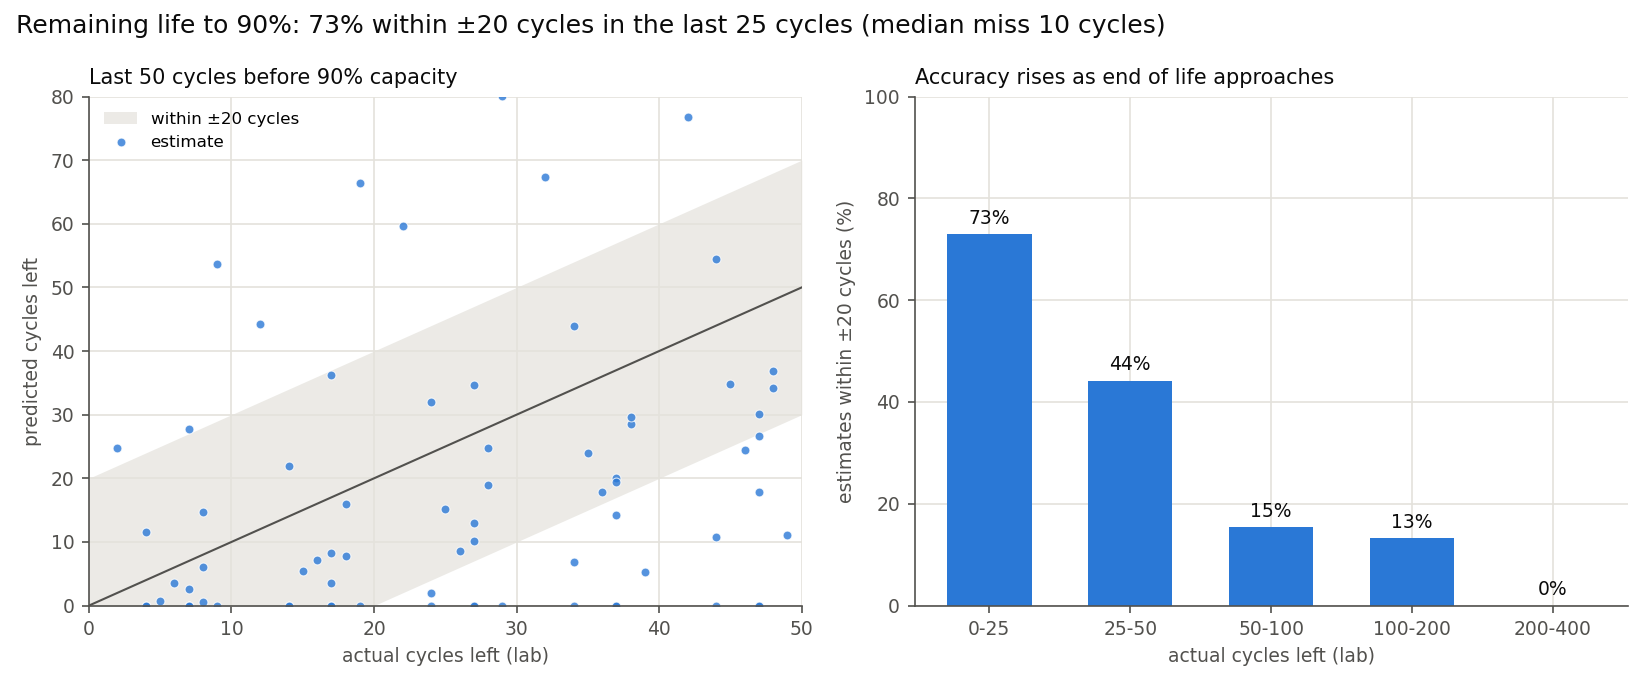
\includegraphics[width=\textwidth]{figures/results_rul.png}
\caption{RUL to 90\% capacity. Left: predicted against actual cycles left in the
last 50 cycles. Right: share of estimates within $\pm$20 cycles by actual
distance to end of life.}
\label{fig:rul}
\end{figure}

\subsection{RUL when complete discharges are rare}
\label{sec:res-sparse}

A driver who seldom fully discharges produces few complete discharges (CS2\_24:
18 in 1{,}617). Four methods were evaluated on the same sparse evidence
(Table~\ref{tab:sparse}). Sparsity is real on the partial-cycling cells and
emulated as one complete discharge in 50 on the constant-current cells.

\begin{table}[t]
\centering
\caption{RUL from sparse complete discharges. None is accurate enough to report.}
\label{tab:sparse}
\begin{tabular}{p{0.42\textwidth}p{0.5\textwidth}}
\toprule
Method & Outcome \\
\midrule
Sparse capacity, standard minimum & refuses every point (never reaches 30) \\
Field SOH trajectory & answers 62\%; median miss 79 cycles when predicting $<$25 \\
Field SOH scaled by the cell's own complete discharges & over-corrects; errors turn late near end of life \\
Sparse capacity, minimum lowered to 5 (post hoc) & 0\% within $\pm$20 cycles; misses late \\
\bottomrule
\end{tabular}
\end{table}

The field-trajectory failure has a clean cause. Near 0.90, field SOH reads a
median 1.1 points below capacity. Because fade near the threshold is slow, that
small bias moves the 0.90 crossing a median 56 cycles early. An SOH error
acceptable as a health figure thus becomes large as a time to threshold. None of
the four is reported; the system refuses RUL for partial-only records and
states that this was tested.

\subsection{When the evidence suffices}
\label{sec:res-suff}

Three questions were fixed before the study, scored at every laboratory check
on 19 cells.

\paragraph{Count does not predict accuracy}
Median error was 0.75\% at 6--10 usable readings and 1.97\% beyond 60. Error
grows with age as the approximation in Eq.~\eqref{eq:soh} drifts, rather than
shrinking with count. A rule of high confidence after a fixed number of
discharges therefore has no support.

\paragraph{Consistency does}
Table~\ref{tab:suff} gives the result. The pooled Spearman correlation between
$u$ and absolute error was 0.48. Within cells it was weaker (median 0.14,
positive in 14 of 19): $u$ chiefly separates unreliable cells and periods rather
than ranking readings within a good one.

\begin{table}[t]
\centering
\caption{Error by the consistency criterion of Eq.~\eqref{eq:u}.}
\label{tab:suff}
\begin{tabular}{lrrcc}
\toprule
Readings & Points & Cells & Median error & 90th percentile \\
\midrule
$u \le 0.01$ (consistent) & 8{,}993 & 16 & 1.3\% & 4.4\% \\
$u > 0.01$ (inconsistent) & 2{,}168 & 13 & 5.1\% & 21.9\% \\
\bottomrule
\end{tabular}
\end{table}

\paragraph{Reference size}
In the study's own scoring, larger references reduced error (1 discharge:
3.6\%; 5: 2.0\%; 10: 1.3\%). On the field-study metric of
Section~\ref{sec:res-field}, however, ten versus five changed the median from
1.681\% to 1.665\%, so the estimator retains five.

\paragraph{Resulting confidence rules}
Capacity-health confidence is assigned as follows:
\begin{itemize}
\item \emph{high}: consistent, fixed window and a beginning-of-life reference;
\item \emph{medium}: consistent, but a learned window or a start-of-log
reference;
\item \emph{low}: inconsistent, reported with the measured 22-point band.
\end{itemize}

\subsection{System integration and refusals}
\label{sec:res-system}

The estimators run inside one pipeline shared by three acquisition paths: CAN
with a DBC definition, a serial bench rig, and research datasets. Every output
is labelled measured, estimated or heuristic and carries its error band.

The bench rig streamed 83 of 83 checksummed frames at a measured 1.000~s
cadence without gaps. Its two sensors have not yet operated in one capture and
no discharge has been recorded, so it validates acquisition, not health
estimation.

Fault injection into a real capture behaved as designed: a corrupted byte failed
its checksum, a NaN field was rejected, a reversed timestamp refused the
capture, and a missing sensor was refused by name. It also exposed one defect,
since corrected: a 999~V reading passed the field range, which is wide so that
packs are admissible. Records outside 0--5~V are now rejected when the source
declares a single cell.

%% ===========================================================================
\section{Discussion}
\label{sec:discussion}

\paragraph{Conditioning moved accuracy; model choice did not}
Across fourteen fitted methods, LOCO differences were smaller than the
uncertainty on any one of them. Three conditioning decisions, by contrast,
changed error by multiples:
\begin{itemize}
\item refusing truncated discharges took the worst cell from 52\% to
${\sim}$10\%;
\item identifying resistance from the load step took the median from 4.3\% to
1.7\% and coverage from 12 to 17 cells;
\item refusing knee windows converted 6.8--12.8\% errors into refusals.
\end{itemize}
For a BMS software layer, the leverage lies in what is measured and how it is
conditioned, not in the regressor that follows.

\paragraph{Reference definitions change conclusions}
Two of our results moved when the reference was made one a BMS can hold. RUL
accuracy fell from 88\% to 73\%, and a partial-discharge reference formed at
discharge 805 produced a 58\% error until the timing gate existed. Validation
should use the reference the deployed system will have; one computed from the
whole record leaks the future.

\paragraph{Threshold crossings amplify small biases}
A 1.1-point SOH bias, unremarkable as a health figure, shifted predicted end of
life by ${\sim}$56 cycles. Any RUL built on an estimated rather than measured SOH
inherits this, and should be evaluated as a time to threshold rather than via
SOH error.

\paragraph{Sufficiency is measurable}
Treating ``enough data'' as a count is intuitive and here wrong, because the
estimator's error is dominated by age-related drift rather than sampling. The
consistency of readings is observable without ground truth and separates 1.3\%
from 5.1\% median error. This gives a BMS layer a principled way to report
``not yet'' for a battery it has never seen. It requires no population model,
because every estimate is relative to the cell's own first discharges.

%% ===========================================================================
\section{Limitations}
\label{sec:limits}

\begin{itemize}
\item \emph{One chemistry family, single cells, constant current.} Packs add
cell-to-cell imbalance, thermal gradients and balancing currents. Dynamic drive
cycles would challenge both the window read and the step-resistance estimate.
The flat plateau of lithium iron phosphate would challenge the window method
directly.
\item \emph{Two cells per partial-cycling band.}
\item \emph{No temperature correction}, since CALCE cycling carries no
temperature channel. A cold cell would read low SOH and high resistance without
having aged.
\item \emph{End of life at 90\% only.}
\item \emph{Apparent resistance.} $R_\mathrm{step}$ depends on the logger's
sample interval; it is comparable within a record, not across loggers.
\item \emph{Drift with age.} Window charge does not scale exactly with capacity,
and error grows over life.
\item \emph{No hardware discharge} has yet been recorded on the bench rig.
\end{itemize}

%% ===========================================================================
\section{Conclusion}
\label{sec:conclusion}

A software layer over a BMS can measure lithium-ion cell health from voltage,
current and time without any model trained on other cells. On 22 CALCE cells it
delivered:
\begin{itemize}
\item capacity health at 1.7\% median error, with every refusal explained;
\item a resistance trend that tracks the laboratory instrument on 19 of 20
cells;
\item partial-discharge capacity health at 3.2--3.4\% on two cells, with a
physical rule that refuses the knee;
\item a remaining-life estimate that, near end of life, behaves as a safe lower
bound.
\end{itemize}
Each output carries a measured error band and is withheld when its evidence is
missing or inconsistent. The consistency criterion that makes that decision was
itself validated against laboratory truth. The outputs that failed validation,
namely fitted models across protocols and RUL from sparse complete discharges,
are refused rather than reported.

%% ===========================================================================
\section*{CRediT authorship contribution statement}
\textcolor{red}{[To be completed.]} \textbf{Naveen Vaidyanathan:}
Conceptualization, Methodology, Software, Validation, Formal analysis,
Investigation, Data curation, Writing -- original draft, Writing -- review \&
editing, Visualization.

\section*{Declaration of competing interest}
\textcolor{red}{[To be completed by the author.]}

\section*{Declaration of generative AI and AI-assisted technologies in the
writing process}
\textcolor{red}{[To be completed by the author, describing honestly how
AI-assisted tools were used in the software, analysis and drafting of this
work, in accordance with the journal's policy. The author must review and edit
all content and take full responsibility for it.]}

\section*{Data availability}
All code, tests and result artifacts are available at
\url{https://github.com/Navvu-gityhub/Behavior-Aware-BMS}. Every number in
this article is regenerated by a named script from committed artifacts
(Appendix~\ref{app:artifacts}). The raw CALCE and NASA data are not
redistributed; download locations are given in the repository.

\section*{Acknowledgements}
\textcolor{red}{[To be completed.]}

\appendix
\section{Provenance of every reported number}
\label{app:artifacts}

\begin{table}[h]
\centering
\small
\begin{tabular}{p{0.16\textwidth}p{0.4\textwidth}p{0.36\textwidth}}
\toprule
Section & Artifact (\texttt{reports/metrics/}) & Script (\texttt{scripts/}) \\
\midrule
\ref{sec:res-bench} & \texttt{benchmark\_results.csv}, \texttt{ablation/} & \texttt{run\_benchmark\_study.py}, \texttt{run\_ablation\_study.py} \\
\ref{sec:res-field} & \texttt{calce\_field\_soh/} & \texttt{run\_field\_soh\_study.py} \\
\ref{sec:res-partial} & \texttt{calce\_partial\_soh/} & \texttt{run\_partial\_soh\_study.py} \\
\ref{sec:res-r} & \texttt{calce\_resistance/} & \texttt{run\_resistance\_study.py} \\
\ref{sec:res-rul} & \texttt{calce\_rul\_horizon\_early\_ref/}, \texttt{error\_bands.csv} & \texttt{run\_rul\_horizon\_study.py}, \texttt{build\_error\_bands.py} \\
\ref{sec:res-sparse} & \texttt{calce\_field\_rul/} & \texttt{run\_field\_rul\_study.py} \\
\ref{sec:res-suff} & \texttt{calce\_sufficiency/} & \texttt{run\_sufficiency\_study.py} \\
Figs.~\ref{fig:track}--\ref{fig:rul} & \texttt{reports/figures/results\_*.png} & \texttt{export\_results.py} \\
\bottomrule
\end{tabular}
\end{table}

\bibliographystyle{elsarticle-harv}
\bibliography{references}

\end{document}
